\chapter{Project Overview}\label{chap:Overview}

The main project description we started to work with was quite short with about 300 words and was also hugely complemented and clarified in meetings with Prof. Weber-Wulff. Nonetheless it contains very important parts that are the foundation of what was built during the project:

\begin{quote}
\enquote{Right. I'm the plagiarism \enquote{huntress}. I've tested plagiarism detection software since 2004. Mostly, they suck. They either don't work, or are a pain to use, or both. I've spent 10 years trying to educate people about plagiarism, and still the media thinks I have a magic secret for discovering plagiarism, as demonstrated on the GuttenPlagWiki and the VroniPlagWiki. What actually happens there is that quite a number of tools are used for preparing texts, discovering possible sources, comparing them, and documenting them. The last part is done by hand and takes an enormous amount of time.

The idea is to set up a Plagiarism Detection Cockpit that integrates all sorts of bits and pieces, but leaves the teacher in command. It is not to be a general test system that spits out a number for every paper submitted, although the integration of as many such systems as possible will be one of the necessary features of the system. There will be a lot of thought needed for the interface design, as there are massive amounts of data that need to be displayed. How can this be compressed and fit on a screen? For example, a barcode-generation needs to be integrated.

The goal will be to provide a tool that easily produces simple-to-read 
documentation and deals with all sorts of nastiness that might 
turn up on the way. The tool must be multi-lingual and open source.
 It would also be cool to integrate some of the little tools such 
 as the Android-based OCR-Scanner that was developed in the SS 2011. 
 I would like for the team to use an agile development methodology 
 so that we can continuiously test with teachers and professors 
 and *Plaggers.

One of the first tasks will be collecting up the computing 
literature on the topic of plagiarism discovery. A wiki needs to 
be set up with links to material (online and offline), comments on 
the papers, and as many navigational indices as possible.}\citep{projectDescription}
\end{quote}

In the beginning the main takeaways we used from this text were:

\begin{itemize}
\item \textbf{no} automated process, \enquote{just} a tool that aids the users workflow
\item needs an open source license
\item multi language support
\end{itemize}

If you read the text carefully though, you may notice that we 
overlooked or at least marginalized some important clues, but you 
will find descriptions of those problems later on in the chapter \nameref{chap:summaryAndOutlook}.

One important information that was only stated during the first project proposal was, that it also needed to be web based.

For the frontend this made the choices of languages and technologies pretty easy, because there are some clear web standards, without much alternatives aside from the version numbers. As we wanted to develop in a future-proof manner and chose to support only from Internet Explorer 8 upwards, this lead us to CSS3 for styling, HTML5 for the markup and JavaScript for client-side scripting. With JavaScript being the only one of those three with a real competitior in \href{http://www.dartlang.org/}{Googles Dart}, but as the browser support is still very weak, 
this wasn't a possibility.

On the server-side however the possibilities for programming languages and platforms are a little bit broader than this. The most
important criterias for us regarding those choices were, that it had to be flexible and already very widespread, because this would be helpful for an open source project to gather a community later on.

From the twenty most used programming languages according to \citet{tiobe} only PHP, Ruby, JavaScript(with \href{http://nodejs.org/}{Node.js}), Java and Python seemed really suitable for web development. Naturally the familiarity and preferences of the team members also played a role in the final decision. We made bad experiences with Java in this area and felt that structuring JavaScript and Python in a big application could be problematic. From the two
languages that were left, the one we had the most experience with and that also has the 
biggest following was PHP, so it made the final cut.

For the \enquote{platform} we only made the decision to use Apache as the web server, because it is the most common\citep{webServers} and it also runs on many different operating systems, so that the real platform choice doesn't need to be made.

As you will see below, the usage of a database was also made in a flexible way. We currently use MySQL, but it should be possible to swap the storage engine easily.

\section{Statistics}

We gathered some data of the state of Unplagged as of July 7th 2012 with the tool \href{http://cloc.sourceforge.net/}{Count Lines of Code(CLOC)}. We know that by no means this can be used as a quality measurement, but we believe that it can give some structural insights and is a good starting point for an introduction of the technical area.


\begin{figure}[!h]
  \centering
\begin{tabular}{lrrr}
\toprule
Language & Files & Comments & Code \\
\midrule
PHP & 3262 & 275579    &     429308 \\
XML & 194 & 0 & 234696 \\
HTML                     &         2645       &     191     &     24684 \\
CSS                      &         1220      &      843     &      7093 \\
Javascript                & 59       &       1932     &      5239 \\
XSD                      &           108     &         6       &    1058 \\
SQL                    &        49        &     58      &      102 \\
C                      &            18           &  16       &      72 \\
make                  &                     4      &       4    &         13 \\
\midrule
Sum: & 4013 & 278629 & 702265 \\
\bottomrule
\end{tabular}
  \caption{Complete measurements including library/framework files}
  \label{tab:completeMeasure}
\end{figure}

The table in figure \ref{tab:completeMeasure} shows the complete(At least according to CLOC) count of files, comment lines and lines of code, that is currently part of Unplagged. It contains also all the code 
that is part of all used libraries or frameworks.

In all the following pie charts the measurements you will see are narrowed down as much as possible\footnote{CLOC was called with the following arguments: perl /cloc-1.56.pl application tests scripts public library/Unplagged --force-lang=html,phtml --exclude-dir=libs} to contain only code that was created by members of the team.

\begin{figure}[!h]
  \centering
    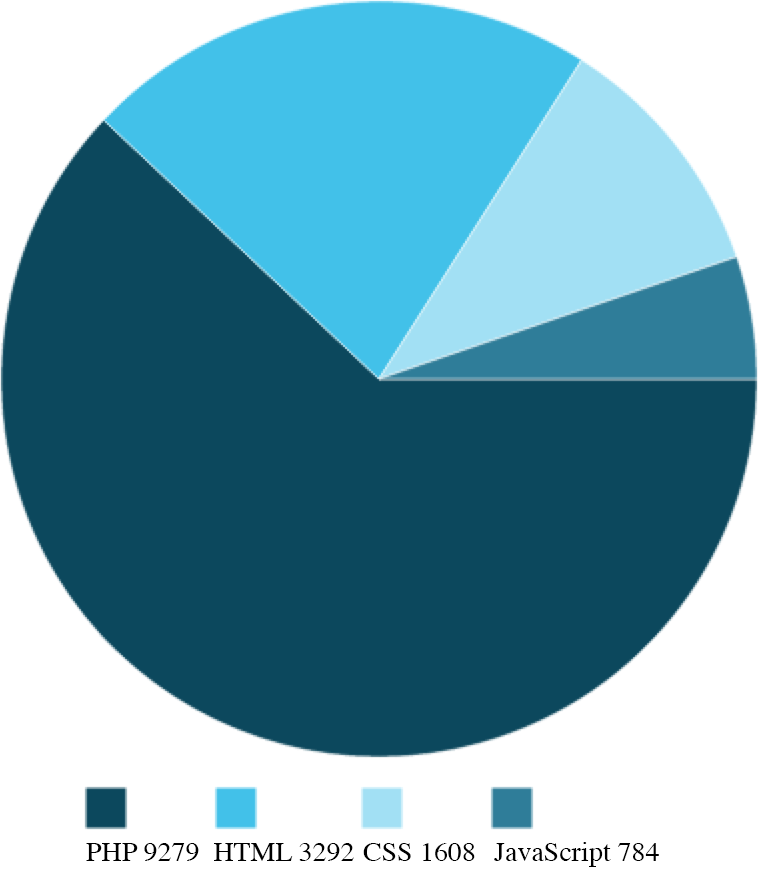
\includegraphics[width=0.55\textwidth]{images/loc.png}
  \caption{Distribution of created lines of code by language.}
  \label{fig:locDistribution}
\end{figure}

As you can see when comparing the numbers in figure \ref{fig:locDistribution} with the table, we are really standing on the shoulders of giants as is often said, with just about 2.1\% of the whole PHP code written by us for example.

\begin{figure}[!h]
  \centering
    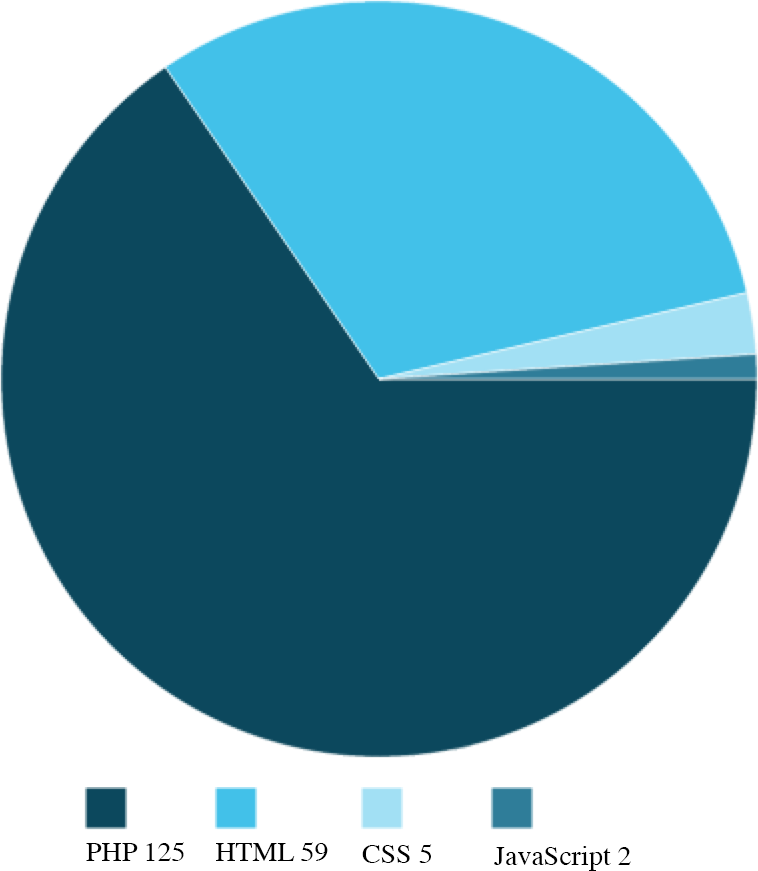
\includegraphics[width=0.55\textwidth]{images/files.png}
  \caption{Distribution of self created files in Unplagged.}
  \label{fig:fileDistribution}
\end{figure}

What could be a bit misleading is the count of HTML files and lines, because they mostly contain some kind of mish-mash of PHP and HTML, including some simple loops to generate reccuring elements.

For the main architecture of the system that lies in the PHP part, we feel that the ratio of 125 files(see figure \ref{fig:fileDistribution}) to 9279 lines of code(see figure \ref{fig:locDistribution}) or ca. 75 lines of actual code per file is a pretty good achievement, as it is at least an indicator of a good software design. For JavaScript and CSS the numbers 
are not that great, but this happened mostly due to performance concerns, because it is 
really desirable to reduce HTTP requests the client has to make.

With comments it's even more complicated to judge the quality by pure numbers of lines,
because they are just there and have no \enquote{understanding ratio} that could be easily measured, but to complete this short excursion into statistical territory: In figure \ref{fig:commentDistribution}, you can see the distribution of comments by language, with PHP again leading the pack by far.

\begin{figure}[!h]
  \centering
    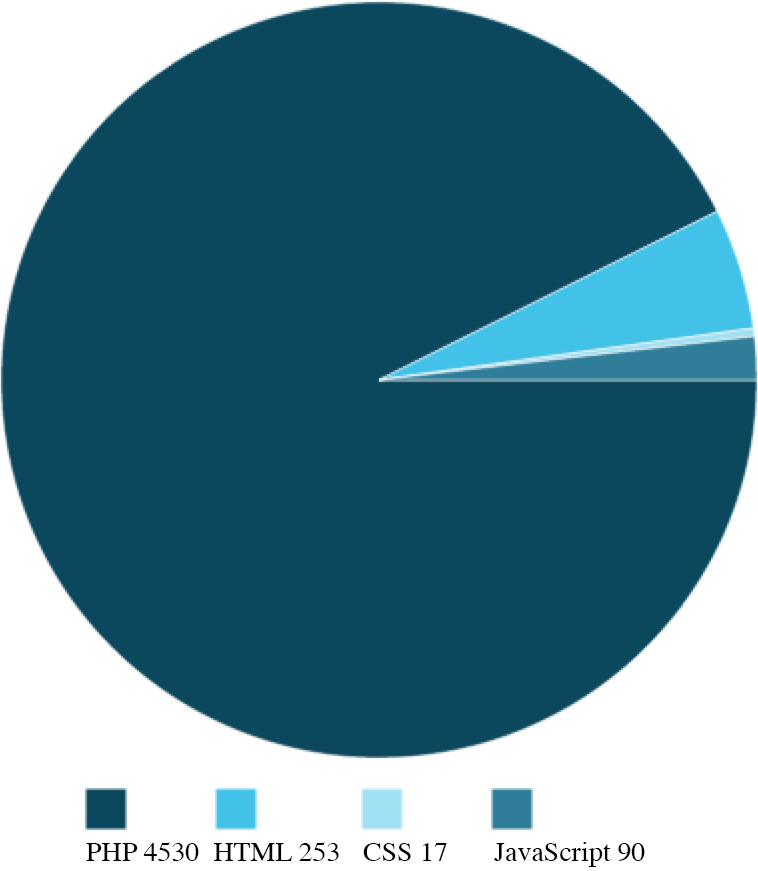
\includegraphics[width=0.55\textwidth]{images/comments.png}
  \caption{Distribution of comment lines by language.}
  \label{fig:commentDistribution}
\end{figure}

\section{Licensing -- GPLv3}

Choosing an open source license was something that was surprisingly difficult for us,
because we never had to do it before and there are so many different possibilites out there with many upsides and downsides.

We eventually decided to use the GNU Public License in version 3(GPLv3). The reasons for this choice are the very widespread usage of it, meaning that many people are already 
familiar with it, the international validity of the specified terms and the \enquote{viral}
character of it, so that any additions and changes to the software also need to be provided 
under the same open source license.

It has therefore the benefit of keeping the possibility to dual-license the system with another proprietary license later on in order to maybe even sell it to organizations who want to include
customizations without making them public, which would be mandatory under the GPLv3.

\section{Project Structure and Technologies}

Over the course of the project we integrated some kind of \enquote{toolbox} of libraries and frameworks, which 
helped us develop faster, more efficient or according to some kind of \enquote{best-practices}
in some areas. 

\subsection{Zend Framework}

\subsection{Doctrine ORM}

\subsection{HTML5 Boilerplate}

\subsection{jQuery}

\subsection{Twitter Bootstrap}

\subsection{Responsive Design}

\subsection{SIM}

\subsection{Tesseract, Imagemagick and Ghostscript}


